\documentclass[a4paper, oneside]{discothesis}

% use utf8 instead of latin1 when using LaTeX in windows
\usepackage[latin1]{inputenc}
\usepackage{mathtools}
\usepackage{comment}
\usepackage{makecell}
\DeclareMathOperator*{\argmax}{\operatorname{argmax}}

%%%%%%%%%%%%%%%%%%%%%%%%%%%%%%%%%%%%%%%%%%%%%%%%%%%%%%%%%%%%%%%%%%%%%%%%%%%%%%%%%%%%%%%%%%%%%%%%%
% DOCUMENT METADATA

\thesistype{Master Thesis}
\title{Adabtive Hierarchical Deep Reinforcement Learning}

\author{Florian Frei}
\email{flofrei@student.ethz.ch}
\institute{Distributed Computing Group \\[2pt]
Computer Engineering and Networks Laboratory \\[2pt]
ETH Z�rich}

% You can put in your own logo here "\includegraphics{...}" or just comment the command
\logo{}

\supervisors{Gino Brunner, Oliver Richter\\[2pt] Prof.\ Dr.\ Roger Wattenhofer}

% You can comment the following two commands if you don't need them
% \keywords{Keywords go here.}
% \categories{ACM categories go here.}

\date{\today}

%%%%%%%%%%%%%%%%%%%%%%%%%%%%%%%%%%%%%%%%%%%%%%%%%%%%%%%%%%%%%%%%%%%%%%%%%%%%%%%%%%%%%%%%%%%%%%%%%

\begin{document}

\frontmatter % do not remove this line
\maketitle

\cleardoublepage

\begin{acknowledgements}
	I thank you.
\end{acknowledgements}


\begin{abstract}
	smart short recapitulation of stuff done
	main work experiments with temporal abstraction and their adaptability 
\end{abstract}

\tableofcontents

\mainmatter % do not remove this line

%Main reference deep learning \cite{goodfellow2016deep}
%Proximal Policy Approximation for OpenAI five \cite{schulman2017proximal}

\chapter{Introduction}
In 2017 an artificial intelligence named Alpha Go \cite{silver2017mastering} beat the worlds known strongest player. This was achieved without using human knowledge but rather only with playing against itself. Hence reinforcement learning has high potential to learn more complex tasks and thus help humans in the next breakthrough in technology. Maybe this comes by enabling neural networks to do temporal abstraction on its objective. Therefore in this work we want to test the \emph{adaptability} and \emph{limitations} of the option-critic architecture from Harb et al. (2017) \cite{harb2017waiting} and the usability of deliberation cost. 

\section*{Background}
The research topic of machine learning is huge and also really old. We don't mention the basics and concentrate on the aspect of deep learning. We recommend the book from Goodfellow et al. (2016) \cite{goodfellow2016deep} as an introduction and we will assume the reader has a basic understanding of its content. Two algorithms worth mentioning is the deep Q-network(DQN) algorithm from Mnih et al. (2015) \cite{mnih2015human} and the asynchronous actor critic(A3C) from Mnih et al. (2016) \cite{mnih2016asynchronous}.

\section*{Related Work}
The idea of using a hierarchy in reinforcement learning to increase efficiency is well established. The first approach was to define macro actions or operators which can be invoked instead of just basic actions. The first three real frameworks which are still used today were proposed in the nineties. To summarize these three major frameworks were the options framework of Sutton et al. (1999) \cite{sutton1999between}, the HAM(hierarchical abstract machines) framework of Parr et al. (1998) \cite{parr1998reinforcement}, and the MaxQ framework of Dietterich (2000) \cite{dietterich2000hierarchical}. This thesis is based on the options framework.

\chapter{Preliminaries}

\section*{Markov Decision Process(MDP)}
A finite discounted MDP $\mathcal{M}$ is a tuple $\mathcal{M} \doteq (\mathcal{S},\mathcal{A},\gamma,r,P)$ encapsulating a state space $\mathcal{S}$, an action space $\mathcal{A}$, a discount factor $\gamma$ where $\gamma \in [0,1)$, a reward function $r(s,a): \mathcal{S} \times \mathcal{A} \to \mathbb{R}$ which maps a state-action pair to a real number and state transition probability function $P(s,a):\mathcal{S} \times \mathcal{A} \to \mathbb{S} $ which maps old states with actions to new states.

\section*{Policy $\pi$}
A policy $\pi(s) : \mathcal{S} \to \mathcal{A} $ is a description of behavior. Meaning in a deterministic setting the action taken is always the same given the same state. In a stochastic setting the policy $\pi(a | s) : \mathcal{S} \times \mathcal{A} \to [0,1]$ is a distribution given a state. This means an action is sampled from this distribution where each action has a probability of getting selected.

\section*{Value Function}
For each action in given state $s$ the environment returns a reward $r(s,a)$. Based on this reward a value function can be defined as follows given start state $s$:
\begin{equation*}
V^{\pi}(s) = \mathbb{E} \left[ \sum_{t=1}^{\infty} \gamma^{t} r_t(s_t,a=\pi(s_t)) \right]
\end{equation*}
This value can be used to compare different policies given start state $s$. With the same concept in mind a value can be calculated when the first action is additionally separated from the rest of the policy. This yields a state-action value function $Q_{\pi}(s,a):\mathcal{S}\times\mathcal{A} \to \mathbb{R}$ which can be used to compare different initial actions $a$ from a given start state $s$.

\section*{$\epsilon$-greedy policy}
Since values can be calculated for given states or state-action pairs we also can define a policy based on these values. A well-known definition is the $\epsilon$-greedy policy which takes with $\epsilon$ probability a random action or else it takes the maximum of the Q-value function.
\begin{equation*}
\pi_{\epsilon} = \begin{cases}
				  a \sim U_{\mathcal{A}} & \text{if} \; 0<p<\epsilon<1 \\
				  \displaystyle \max_{a \in \mathcal{A}}{Q(s,a)} &\text{if} \;  0<\epsilon<p<1 	
			     \end{cases} \qquad p \sim U_{(0,1)}
\end{equation*}

\section*{Policy gradient methods}
In general a policy $\pi$ is dependent on parameters $\theta$ which for example describe the distribution. Hence the goal in reinforcement learning is to optimize the policy parameters $\theta$ so that the expected return
\begin{equation*}
 J (\theta) = \mathbb{E} \left[ \sum_{t=1}^{\infty} \gamma^{t} r_t \right]
\end{equation*}
is maximized where $\gamma \in [0,1]$ is the discount factor. This can be accomplished by using the gradient update rule:
\begin{equation*}
\theta_{t+1} = \theta_{t} + \alpha_t \cdot \nabla_{\theta} J(\theta) \big|_{\theta=\theta_t} 
\end{equation*} 
where $\alpha_t$ is the learning rate. The main problem in policy gradient methods is to obtain a good estimator of the policy gradient $\nabla_{\theta} J(\theta) \big|_{\theta=\theta_t}$. $\alpha_t$ is often refereed to as a hyper-parameter where the best value has to be searched over $[10^{-1},10^{-5}]$ given an environment and algorithm. For a more rigorous explanation of policy gradient methods we refer to Williams (1992) \cite{williams1992simple} and Peters et al. (2008) \cite{peters2008reinforcement}


\section*{Option-critic}
Learning with temporally abstract actions, named options, from Sutton et al. (1999) \cite{sutton1999between} depend on past decisions. Options are in essence encapsulated policies and thus also a super-policy is required who decides which options gets control in a given state. The last piece needed is a function which describes when a sub-policy should terminate itself and give control back to the super-policy. Mathematically described an option consists of three components. A stochastic sub-policy $\pi_{\omega}:\mathcal{S}\times \mathcal{A} \to [0,1]$ which represents the behavior of an option $\omega$, a termination function $\beta: \mathcal{S} \to [0,1]$ which describes the probability of terminating option $\omega$ given state $s$, and an initiation set $\mathcal{I}_{\omega} \subset \mathcal{S}$ containing the all states from which an option $\omega$ can start from. Last but not least the super-policy $\pi_{\Omega}: \mathcal{S} \times \Omega \to [0,1]$ where $\Omega$ is the set of options. The super-policy is chosen to be $\epsilon$-greedy using the $Q$-value function in this case an a option-state value function. For options the normal MDP has to be extended to a semi-Markov decision process(SMDP) \cite{puterman2014markov} in which the transition time between two decision points is a random variable and shown in figure \ref{fig:mdp_vs_smdp}.\\
\begin{figure}
\includegraphics[scale=0.9]{options_over_mdp.pdf}
\caption{Comparison of time transitions in MDP's and SMDP's}
\label{fig:mdp_vs_smdp}
\end{figure}
\noindent The option-critic architecture \ref{fig:option_critic_arch} is similar to the actor-critic algorithm hence the name. For a complete mathematical derivation we refer to Bacon et al. (2017) \cite{bacon2017option}. We only highlight the resulting equations. In this architecture the super-policy acts $\epsilon$-greedy based on $Q$-values learned by $Q$-learning. The super-policy selects an option which is as already mentioned just a stochastic sub-policy which returns basic actions until termination. As one can imagine this model allows in a sense temporally extended sub-strategies. When the termination function is set to $1.0$ for all states the algorithm collapses to basic actions but chosen indirectly over the super-policy and the option-state value function. The initiation set is generally given by the set of all states meaning any option can start from any state.\\
\begin{figure}
\includegraphics[scale=1.1]{option_critic_arch.pdf}
\caption{Depiction of the option-critic architecture}
\label{fig:option_critic_arch}
\end{figure}
\noindent The function for the $Q$-values used by the super-policy is given by the following equation:
\begin{equation*}
Q_{\Omega}(s,\omega) = \sum_{a} \pi_{\omega,\theta}(a|s) Q_{U}(s,\omega,a)
\end{equation*}
It is simply the expectation over all actions an option $\omega$ can take and a corresponding state-option-action value given by the sub-policies. The state-option-action value function is defined as follows:
\begin{gather*}
Q_{U}(s,\omega,a) = r(s,a) + \gamma \sum_{s'} P(s'|s,a) U(\omega,s') \\
U(\omega,s') = (1-\beta_{\omega,\vartheta}(s'))Q_{\Omega}(s',\omega) + \beta_{\omega,\vartheta}(s') V_{\Omega}(s')
\end{gather*}
where $U(\omega,s')$ is an utility term calculated for the two cases. When the option $\omega$ does not terminate we use the $Q$-value from before for the new state $s'$ otherwise use an estimation $V_{\Omega}(s')$ over all options. Note that this recursion has the same structure as the Bellman equation and hence TD estimation is also applicable. The derivation is the same as before by taking the gradients with respect to $\theta$ and $\vartheta$ as to maximize the expected return for all states. 

\subsection*{Intra-option gradient}
First we show the policy gradient of the sub-policies also called intra-option gradient. 

\begin{gather*}
\rho(\theta) = \mathbb{E}\left[  \sum_{t=1}^{\infty} \gamma^{t-1} R_t \bigg| s_0,\omega_0,\Omega \right]=Q_{\Omega}(s_0,\omega_0) \\
\frac{\partial Q_{\Omega}(s,\omega) }{\partial \theta} = \sum_{s} \sum_{\omega} d_{\Omega}(s,w) \sum_{a} \frac{\partial \pi_{\omega,\theta}(a|s) }{\partial \theta } Q_{U}(s,\omega,a)
\end{gather*}
Note that here the same old trick with the log transformation and using action sampling can be made. Also $d_{\Omega}(s,w)$ is again the discounted weighting of states along an option.

\subsection*{Termination gradient}
Next is the gradient from the termination where we want to maximize the utility function. 
\begin{gather*}
\rho(\vartheta) = \mathbb{E}\left[  \sum_{t=1}^{\infty} \gamma^{t-1} R_t \bigg| s',\omega,\Omega \right]=U(s',\omega) \\
\frac{\partial U_{\omega, s'} }{\partial \vartheta} = \sum_{\omega'} \sum_{s''} d_{\Omega}(s',\omega ) \frac{\partial \beta_{\omega',\vartheta}(s'') }{\partial \vartheta} \left( V_{\Omega}(s'') - Q_{\Omega}(s'',\omega') \right)
\end{gather*} 
where $A_{\Omega}(s',\omega) = Q_{\Omega}(s',\omega')- V_{\Omega}(s') $ is the already seen advantage function with respect to option $\omega$. This makes intuitively sense because $V_{\Omega}(s')$ is estimated from all options. Hence when there is a better option this value is higher than the current state-option value and the advantage function is negative. Thus the sum is positive and we increase the termination probability. The same logic applies for the reverse case where we want to decrease the termination probability in case the state-option value is higher than value estimation from all options. \\
In case that the action space is to large and therefore $N_{\Omega} \cdot N_{\mathcal{A}}$ huge we can estimate $Q_U$ from $Q_{\Omega}$ as shown below:
\begin{equation*}
Q_{U}(s,\omega,a) = r(s,a) + \gamma \sum_{s'} P(s'|s,a) U(\omega,s')=r(s,a)+\gamma \mathbb{E}_{s' \sim P } \left[ U(\omega,s') \big| s,a \right]
\end{equation*}


\section*{Deliberation cost}
As apparent from the figure \ref{fig:delib_cost} at each decision point, marked with a white circle, an additional cost is added. This penalizes fast changes between options. Mathematically this is done by defining an immediate cost function $c(s,\omega,a,s',\omega')$ and a corresponding deliberation cost function $D_{\theta}(s,\omega)$. 
\begin{figure}[!ht]
\includegraphics[scale=0.7]{option_critic_delib_cost.pdf}
\caption{Structure of deliberation cost model}
\label{fig:delib_cost}
\end{figure}
\noindent Without going into the rigorous derivation from Harb et al. (2017) \cite{harb2017waiting} we show the new equations.
\begin{gather*}
\rho(\vartheta) = \mathbb{E}\left[  \sum_{t=1}^{\infty} \gamma^{t-1} ( R_t - \eta c(s,\omega,a,s',\omega') ) \bigg| s',\omega,\Omega \right]\\
\frac{\partial U_{\omega, s'} }{\partial \vartheta} = \sum_{\omega'} \sum_{s''} d_{\Omega}(s',\omega ) \frac{\partial \beta_{\omega',\vartheta}(s'') }{\partial \vartheta} \left( V_{\Omega}(s'') - Q_{\Omega}(s'',\omega') + \eta \right)
\end{gather*}
Thus one can see that a margin $\eta$ was introduced in the gradient. This allows us to tilt the termination of an option in both directions. For example when the margin is high in comparison to the reward the system will use a chosen option for longer periods of time. A negative $\eta$ motivates the system to change more between given options. 

\begin{comment}
% Start writing here
\chapter{Motivation}
The human capability to learn abstract concepts is well-known but not well understood. Our brain is the most complex organ in our body and its size is the most significant difference to other species. It allows us to be self-aware and defines our individuality. Hence it could be of significant importance to understand how it works for creating artificial intelligence. One aspect of it is the brains capability of high level abstraction. This could be temporal or objective in nature. Meaning that we learn automatically to tackle difficult tasks by dividing them into manageable subtasks. Additionally the function of dopamine allows us to handle delayed gratification. Meaning that for example no immediate reward is needed for pursuing a goal in life. The journey is a sufficient inner motivator regardless if we can reach the set goal. The high complexity of games in the world today such as League of Legends, Dota 2 or Starcraft require a more sophisticated abstraction of the strategy in order to win. Recently they achieved more than human level performance in Dota 2 with training a neural network over half a year but no abstraction levels were used. Thus it is important to better understand abstraction such that it is possible to incorporate abstraction into neural networks to allow better performance. 

\chapter{Introduction}
%Reinforcment Learning
\section*{Reinforcement Learning}
Reinforcement Learning(RL) is besides supervised and unsupervised learning one of the big three themes in machine learning. Without going into details this research field is mostly based on the theory of Markov Decision Processes. There are other types of approaches worth mentioning but we don't want to go into to much detail. For the interested reader or for a complete beginner in this kind of field we refer to we refer Sutton et al. (1998) \cite{sutton1998introduction} and Kaelbling et al. (1996) \cite{kaelbling1996reinforcement} where most on theory and history of this research field with all references can be found.\\
In this work we concentrate on one subfield of reinforcement learning namely hierarchical reinforcement learning. We think a good start where most frameworks are well summarized is in Barto et al.(2003) \cite{barto2003recent} and it also gives a brief introduction to the theory of Markov Decision Processes abbreviated as MDP. For the interested reader which is not particularly fond of reading papers we refer to video course by David Silver free available online on youtube.

\section*{Hierarchical Reinforcement Learning}
%Hierarchical reinforcement learning
The idea of using a hierarchy in reinforcement learning to increase efficiency is well established. The first approaches was to define macro actions or operators which can be invoked instead of just basic actions. The first three real frameworks which are still used today were proposed in the nineties. To summarize these three major frameworks were the options framework of Sutton et al. (1999) \cite{sutton1999between}, the HAM(hierarchical abstract machines) framework of Parr et al. (1998) \cite{parr1998reinforcement}, and the MaxQ framework of Dietterich (2000) \cite{dietterich2000hierarchical}. This thesis is based on the options framework and hence we concentrate only on this type of framework but this does not mean the others are not worth consideration.

\section*{Deep Reinforcement Learning}
Another big aspect in the development of machine learning is due to the rapid improvement of the hardware. More memory and CPU capacity allows faster exploration and tackling more complex tasks. This allowed the realization of neural networks and hence the field of deep reinforcement learning. For a reader which never heard of neural networks we refer to Funahashi (1989) \cite{funahashi1989approximate} where the theory and research references can be found. Neural networks form the basis of most deep reinforcement algorithms today and are used extensively. 

%Bad start reference to randomly sampled replay buffer in RL
%A good starting point into this topic is the work of Mnih et al. (2015) \cite{mnih2015human} which shows that a high level of control can be achieved. 
The state of the art algorithm A3C(asynchronous advantage actor critic) can be found in Mnih et al.(2016) \cite{mnih2016asynchronous} which is often used as a baseline to compare the performance of new developed techniques and algorithms.

% The toolkit we use to compare algorithms fairly on different environments is given by the OpenAI gym from Brockman et al. \cite{brockman2016openai} and will be used as a base in this work to implement our own environments. \\
%To implement neural networks we refer to two libraries namely the overworked theano framework \cite{bergstra2011theano} from Bastien et al. (2012) \cite{bastien2012theano} and tensorflow from Abadi et al. (2016) \cite{abadi2016tensorflow}. In this work we will exclusively use tensorflow in python.
%In this work we concentrate on the proposed hybrid algorithm between the options framework and asynchronous advantage actor critic named option critic from \cite{harb2017waiting} where a deliberation cost was additionally introduced.

\chapter{Preliminaries}
%For the complete theory on MDP's we refer to the literature.
\section*{Markov Decision Process}
Most theory of reinforcement learning research is based on Markov Decision Processes(MDP) since it provides the simplest framework which allows us to study basic algorithms and their properties. A finite discounted MDP $\mathcal{M}$ is a tuple $\mathcal{M} \doteq (\mathcal{S},\mathcal{A},\gamma,r,P)$ encapsulating a state space $\mathcal{S}$, an action space $\mathcal{A}$, a discount factor $\gamma$ where $\gamma \in [0,1)$, a reward function $r(s,a): \mathcal{S} \times \mathcal{A} \to \mathbb{R}$ which maps a state-action pair to a real number and state transition probability function $P(s,a):\mathcal{S} \times \mathcal{A} \to \mathbb{S} $ which maps old states with actions to new states.\\
A policy $\pi(s) : \mathcal{S} \to \mathcal{A} $ is a description of behavior. Meaning in a deterministic setting the action taken is always the same given the same state. In a stochastic setting the policy $\pi(a | s) : \mathcal{S} \times \mathcal{A} \to [0,1]$ is a distribution given a state. This means an action is sampled from this distribution where each action has a probability of getting selected.

\section*{Value Function}
Since a reward can be assigned to each state a value function can be calculated from start state $s$ with a given stochastic policy as follows:
\begin{equation*}
V^{\pi}(s) = \mathbb{E} \left[ \sum_{t=1}^{\infty} \gamma^{t} r_t(s_t,a=\pi(s_t)) \right]
\end{equation*}
This value can be used to compare different policies given start state $s$. With the same concept in mind a value can be calculated when the first action is additionally separated from the rest of the policy. This yields a state-action function $Q_{\pi}(s,a):\mathcal{S}\times\mathcal{A} \to \mathbb{R}$ which can be used to compare different initial actions $a$ from a given start state $s$.

\section*{Bellman Equation}
Now instead looking at the whole trajectory of a policy the Bellman equation \eqref{eq:bellman} from \cite{bellman1956dynamic} (1956) allows one to view it in a recursive manner using the value function as follows:
\begin{equation}
\label{eq:bellman}
V^{\pi} (s)= r(s,a=\pi(s)) + \gamma \sum_{s' \in \mathcal{S}}^{}{ P(s'|s,a=\pi(s)) V^{\pi}(s') }
\end{equation}
In the stochastic setting when the policy follows a distribution and every event is possible the equation can be rewritten as follows:
\begin{equation}
\label{eq:bellman2}
V^{\pi} (s)= \sum_{a}^{}{\pi(a | s)} \left( r(s,a) + \gamma \sum_{s'}^{}{ P(s'|s,a) V^{\pi}(s') } \right) 
\end{equation}
This equation was already usable in dynamic programming. Two major algorithms using Bellman equation were value iteration and policy iteration from Howard (1964) \cite{howard1964dynamic} which could solve successfully MDP's. In value iteration the algorithm acts under an implicit policy such as $\epsilon$-greedy for example and the value function is learned through the state-action function. 
\begin{gather*}
Q_{t+1}(s,t) = r(s,a) + \gamma \sum_{s'}^{}{P(s'|s,a)V_{t}(s)} \\
V_{t+1}(s) = \max_{a} Q_{t+1}(s,a)
\end{gather*}
Whereas in policy iteration a random policy $\pi$ is initialized and then learned stepwise using the value function but not the state-action function.
\begin{gather*}
V^{\pi_t}_{t+1}(s) = r(s,\pi_t(s))+\gamma \sum_{s' \in \mathcal{S}}^{}{P(s'|s,\pi_t(s))V^{\pi_t}_{t+1}(s')}\\
\pi_{t+1}(s) = \argmax_{a} \left( r(s,a) + \gamma \sum_{s'}^{}{P(s'|s,a)V^{\pi_t}_{t+1}(s')} \right)
\end{gather*}

\section*{Temporal Difference}
As one can imagine in reinforcement learning the Bellman equation allows different lengths of recursion. An algorithm using the whole trajectory in an environment are categorized under Monte Carlo methods. The alternative is Temporal Difference (TD) \cite{sutton1988learning} methods which use the Bellman equation and instead of calculating the expectation they estimate the difference from sampling. Hence the temporal difference error resulting is written as:
\begin{equation*}
\operatorname{TD}(0) = R(s,\pi(s))+\gamma V_{\pi}(s') -\gamma V_{\pi}(s) 
\end{equation*}
Notice that $s'$ was sampled from the transition probabilities and can be looked at as a zero order scheme. One can repeat the process and use the same equation to approximate the next value $V_{\pi}(s')$ and so forth. Thus arbitrary recursion schemes can be chosen for this approximation which is a design decision depending on the environment or problem respectively.

\section*{On-policy vs off-policy}
In this recursion we only talked about improving the value function but we are also interested in improving the policy $\pi$ along the way. This can be done in two manners namely on-policy or off-policy. On-policy means that only one policy is used and directly improved with the environment. Off-policy means that there are two policies. One used for exploration with generates data whereas the other policy uses this data to improve itself. Since the policies have different acting distributions sampling methods like importance sampling has to be used to eliminate bias from the action and state samples. This means that in the off-policy case an experience buffer is filled with transitions and then sampled from it to improve the policy.

\section*{SARSA and Q-Learning}
An example for an on-policy algorithm is SARSA \cite{rummery1994line} which stands abbreviated for state action reward state action meaning it uses one transition and the next action to approximate the TD-error. The policy used is $\epsilon$-greedy based on the state-action function $Q$. Meaning with probability $\epsilon$ a random action is taken otherwise the action with the maximum $Q$-value is used. The counterpart to SARSA using off-policy updates is Q-Learning \cite{watkins1992q}.

\section*{REINFORCE}
As we have seen either $\epsilon$-greedy policy was used based on action-value function $Q(s,a)$ to act or another entire policy based on experience. The functions $V(s)$ and $Q(s,a)$ helped to decide which actions are better in the environment in given state and hence improve the policy. But the policy also can be learned directly and are named policy gradient methods. The first method introduces was REINFORCE from Williams (1992) \cite{williams1992simple} where a whole trajectory like in the Monte Carlo method was utilized to improve the policy. The objective is still to maximize the expected cumulative reward.
\begin{equation*}
\rho(s) = \mathbb{E} \left[ \sum_{t=1}^{\infty}{\gamma^{t-1} R_t \Bigg| s} \right]
\end{equation*}
When we define $\tau$ as a complete trajectory and $R(\tau)$ as the reward corresponding to this trajectory the equation can be reformulated as:
\begin{equation*}
\rho(s) = \sum_{\tau}^{}{P_{\theta}(\tau) R(\tau)}
\end{equation*}
where $\theta$ represent the parameters of our policy $\pi$. Instead of using the whole trajectory one can again use an value estimation. This can be learned with TD and reformulated as maximizing:
\begin{equation*}
\rho(s) = \mathbb{E} \left[ \sum_{t=1}^{\infty}{\gamma^{t-1} R_t \Bigg| s} \right] = \sum_{a}^{}{\pi(a|s)Q^{\pi}(s,a)=V^{\pi}(s)}
\end{equation*}
We will not go into detail for the derivation and refer to Sutton et al. (2000) \cite{sutton2000policy} and just present the resulting gradient.
\begin{equation*}
\frac{\partial V^{\pi}(s)}{\partial \theta} = \sum_{x}^{}{d^{\pi}(x)} \sum_{a}^{}{\frac{\partial \pi(a|x) }{\partial \theta} Q^{\pi}(x,a)} 
\end{equation*}
where $d^{\pi}(s)$ is defined as the discounted weighting of states encountered starting at some state $s_0$. In practice most algorithms use $d^{\pi}(x)$ as a stationary distribution which results in an expectation over states. Additionally a baseline is added to reduce variance and together with the log transformation trick the sum can be reduced as follows:
\begin{gather*}
\frac{\partial V^{\pi}(s)}{\partial \theta} = \sum_{s}^{} d^{\pi}(s) { \sum_{a}^{} { \frac{\partial \pi(a|s) }{\partial \theta}  \left[ Q^{\pi}(s,a) - V(s) \right] } } \\
=\sum_{s}^{}{d^{\pi}(s)} \mathbb{E} \left[  \frac{\partial \log{ \pi(a|s) } }{\partial \theta} \left( Q^{\pi}(s,a) - V(s) \right) \right]
\end{gather*}
Note that $V(s)$ in the expectation does not contribute anything so $A(s,a) = Q^{\pi}(s,a) - V(s)$ is often used and known as advantage function. 

\section*{Actor-critic}
The actor-critic algorithm is composed of an actor which learns a policy and a critic which learns a value function. The policy is learned similar to REINFORCE but learned with the value function instead of a sample trajectory. The value function off the current policy is learned via TD approximation. The resulting equations are listed below.  
\begin{gather*}
\frac{\partial \rho}{\partial \vartheta} = \sum_{s} d^{\pi}(s) \sum_{a} \frac{\partial \pi(s,a)}{\partial \vartheta } Q^{\pi}(s,a)= \sum_{s} d^{\pi}(s) \mathbb{E}_a \left[  \frac{\partial \log(\pi(a|s) ) }{\partial \vartheta } Q^{\pi}(s,a) \right] \\
\frac{\partial Q(s,a)}{\partial \theta} = \frac{\partial \left( R(s,a) + \gamma \mathbb{E}_{s'\sim P(s'|s,a)}[V(s')]-Q(s,a) \right)^2 }{\partial \theta} = - \sigma \ast \frac{\partial Q(s,a)}{\partial \theta}
\end{gather*}

\includegraphics[scale=1.3]{actor_critic_arch.pdf}

The next step is to incorporate temporal abstraction into an algorithm. This is no longer possible with simple MDP's and thus the concept was generalized to Semi Markov Decision Processes(SMPD) and we refer to \cite{puterman2014markov} for further reading.

\TODO{SMPD graphic}

\section*{Option-critic}
This is needed since options in the options framework from Sutton et al. (1999) \cite{sutton1999between} depend on past decisions. Options are in essence encapsulated policies and thus also a super-policy is required who decides which options gets control in a given state. The last piece needed is a function which describes when a sub-policy should terminate itself and give control back to the super-policy. Mathematically described an option consists of three components. A stochastic sub-policy $\pi_{\omega}:\mathcal{S}\times \mathcal{A} \to [0,1]$ which represents the behavior of an option $\omega$, a termination function $\beta: \mathcal{S} \to [0,1]$ which describes the probability of terminating option $\omega$ given state $s$, and an initiation set $\mathcal{I}_{\omega} \subset \mathcal{S}$ containing the all states from which an option $\omega$ can start from. Last but not least the super-policy $\pi_{\Omega}: \mathcal{S} \times \Omega \to [0,1]$ where $\Omega$ is the set of options. The super-policy can again be an $\epsilon$-greedy policy.%but now we act greedily based on the estimated $Q$-value belonging to the options. 

\includegraphics[scale=1.3]{option_critic_arch.pdf}

The option-critic architecture is similar to the actor-critic algorithm hence the name. For a complete mathematical derivation we refer to Bacon et al. (2017) \cite{bacon2017option} where everything can be found and we only highlight the resulting equations. In this architecture the super-policy acts $\epsilon$-greedy based on $Q$-values learned by $Q$-learning. The super-policy selects an option which is as already mentioned just a stochastic sub-policy and returns basic actions until termination. As one can imagine this model allows in a sense temporally extended sub-strategies. When the termination function is to high for all states the algorithm collapses to basic actions but chosen indirectly over options. The initiation set is generally given by the set of all states meaning any option can start from any state. The function for the $Q$-values used by the super-policy is given by the following equation:
\begin{equation*}
Q_{\Omega}(s,\omega) = \sum_{a} \pi_{\omega,\theta}(a|s) Q_{U}(s,\omega,a)
\end{equation*}
It is simply the expectation over all actions an option $\omega$ can take and a corresponding state-option-action value given by the sub-policy. The state-option-action value function is defined as follows:
\begin{gather*}
Q_{U}(s,\omega,a) = r(s,a) + \gamma \sum_{s'} P(s'|s,a) U(\omega,s') \\
U(\omega,s') = (1-\beta_{\omega,\vartheta}(s'))Q_{\Omega}(s',\omega) + \beta_{\omega,\vartheta}(s') V_{\Omega}(s')
\end{gather*}
where $U(\omega,s')$ is an utility term calculated for the two cases. When the option $\omega$ does not terminate we use the $Q$-value from before for the new state $s'$ otherwise use an estimation $V_{\Omega}(s')$ over all options. Note that this recursion has the same structure as the Bellman equation and hence TD estimation is also applicable. The derivation is the same as before by taking the gradients with respect to $\theta$ and $\vartheta$ as to maximize the expected return for all states. 

\subsection*{Intra-option gradient}
First we show the policy gradient of the sub-policies also called intra-option gradient. 

\begin{gather*}
\rho(\theta) = \mathbb{E}\left[  \sum_{t=1}^{\infty} \gamma^{t-1} R_t \bigg| s_0,\omega_0,\Omega \right]=Q_{\Omega}(s_0,\omega_0) \\
\frac{\partial Q_{\Omega}(s,\omega) }{\partial \theta} = \sum_{s} \sum_{\omega} d_{\Omega}(s,w) \sum_{a} \frac{\partial \pi_{\omega,\theta}(a|s) }{\partial \theta } Q_{U}(s,\omega,a)
\end{gather*}
Note that here the same old trick with the log transformation and using action sampling can be made. Also $d_{\Omega}(s,w)$ is again the discounted weighting of states along an option.

\subsection*{Termination gradient}
Next is the gradient from the termination where we want to maximize the utility function. 
\begin{gather*}
\rho(\vartheta) = \mathbb{E}\left[  \sum_{t=1}^{\infty} \gamma^{t-1} R_t \bigg| s',\omega,\Omega \right]=U(s',\omega) \\
\frac{\partial U_{\omega, s'} }{\partial \vartheta} = \sum_{\omega'} \sum_{s''} d_{\Omega}(s',\omega ) \frac{\partial \beta_{\omega',\vartheta}(s'') }{\partial \vartheta} \left( V_{\Omega}(s'') - Q_{\Omega}(s'',\omega') \right)
\end{gather*} 
where $A_{\Omega}(s',\omega) = Q_{\Omega}(s',\omega')- V_{\Omega}(s') $ is the already seen advantage function with respect to option $\omega$. This makes intuitively sense because $V_{\Omega}(s')$ is estimated from all options. Hence when there is a better option this value is higher than the current state-option value and the advantage function is negative. Thus the sum is positive and we increase the termination probability. The same logic applies for the reverse case where we want to decrease the termination probability in case the state-option value is higher than value estimation from all options. \\
In case that the action space is to large and therefore $N_{\Omega} \cdot N_{\mathcal{A}}$ huge we can estimate $Q_U$ from $Q_{\Omega}$ as shown below:
\begin{equation*}
Q_{U}(s,\omega,a) = r(s,a) + \gamma \sum_{s'} P(s'|s,a) U(\omega,s')=r(s,a)+\gamma \mathbb{E}_{s' \sim P } \left[ U(\omega,s') \big| s,a \right]
\end{equation*}
\TODO{pseudo code for option critic?}

\subsection*{Regularization}

As often used in state of the art algorithms some regularization is added to some gradients. This can prevent over-fitting to a local optimum by adding randomness to actions such as in entropy regularization. In regard to the termination gradient a small constant term is added since using $\epsilon$-greedy super-policy leads mostly to termination probability of 100\%. This is caused by the value function since
\begin{gather*}
V(s) = \displaystyle \max_{\omega} Q_{\Omega}(s',\omega)
\intertext{and hence}
Q_{\Omega }(s',\omega) - \max_{\omega} Q_{\Omega}(s',\omega) \leq 0 \\
\intertext{and thus the new termination gradient is given by}
\frac{ \partial \beta_{\omega,\vartheta(s')} }{\partial \vartheta} \left( Q_{\Omega}(s',\omega) - \max_\omega Q_\Omega(s,\omega) + \eta_\beta \right)
\end{gather*}
and therefore we allow $\eta_\beta$ margin error between the maximum $Q$-value and the current one given with option $\omega$. As already mentioned there could be a problem with the options where their policy get stuck in a deterministic action distribution. To counter this behavior an entropy is added to the intra-option gradient as shown in the A3C algorithm in Mnih et al. (2016) \cite{mnih2016asynchronous} The entropy is calculated as follows:
\begin{gather*}
H( \pi_{\omega,\theta}(\cdot |s) ) = -\sum_{a} \pi_{\omega,\theta}(a|s)\log(\pi_{\omega,\theta}) \\
\intertext{And hence the new gradient has the following form:}
\frac{\partial Q_{\Omega}(s,\omega) }{\partial \theta} = \frac{\partial \log(\pi_{\omega,\theta}(a|s) )}{\partial \theta} Q_U(s,\omega,a) + \eta_H \cdot \frac{\partial H( \pi_{\omega,\theta}(\cdot |s) )}{\partial \theta}
\end{gather*}

\subsection*{Deliberation Cost}

\chapter{Implementation}
\end{comment}
\section*{Implementation details}
K. Miyoshi re-implemented \cite{miyoshigithubunreal} the UNREAL version based on the paper of Jaderberg et al. (2016) \cite{jaderberg2016reinforcement}. This paper extended A3C algorithm from Mnih et al (2016) \cite{mnih2016asynchronous} with unsupervised auxiliary tasks. His implementation was tested on the DeepMind Lab \cite{beattie2016deepmind}. We used this re-implementation from K. Miyoshi where he also used tensorflow but changed the algorithm to Asynchronous Advantage Option Critic(A2OC) from Harb et al. (2017) \cite{harb2017waiting} and added our own environment. To implement the environment we used the OpenAI gym toolkit from Brockman et al. \cite{brockman2016openai}. The original A2OC from Harb \cite{harbgithuba2oc} uses the thenao framework for neural networks hence it could only be used as a reference.
%(ALE) \cite{brockman2016openai} DeepMind Lab \cite{beattie2016deepmind}

\subsection*{Environment}
For fast evaluation circumvent GPU usage we used an easy two dimensional grid world. There are only three features, namely an empty cell represented as $0.$, the agent position represented as $1.0$ and the goal position represented as $2.0$. The goal for the agent is to reach the goal. After each environment reset the positions of the agent and the goal are uniformly sampled but will never collide. The environment is later extended to also include a key represented with $3.0$ which has to be picked up first in order to reach the goal. \cite{flofreigithubmaze}

\subsection*{Neural Networks}
As already mentioned we used the well-established tensorflow library from Abadi et al. (2016) \cite{abadi2016tensorflow} to implement our neural networks. Given $N_{\omega}$ options we need for A2OC total of $N_{\omega}+3$ networks. Each options has its own neural network and hence we can test mixed models of different depth against each other. The rest is used for the termination model, the Q-value model and the convolution layer. Before the input gets fed into the convolution layer the input is rescaled to $[0,1]$ as it is ueblich when using convolution with filters. In the figure we depict the flow of information but with correct representations of the networks.

\begin{figure}
\includegraphics[scale=0.65]{option_critic.pdf}
\label{fig:option_critic_nn}
\caption{Flow of information in option-critic architecture including showing the neural networks}
\end{figure}

\subsection*{Convolution network}
Since our world is relatively simple we choose one layer of convolution followed by two fully connected layers. The number of filters we choose was $64$ and the filter size was chosen the same as the world size. Meaning a $4 \times 4$ grid world gets a $4 \times 4$ filter since we didn't wanted to loose any information. We used padding such that the dimension stays the same meaning an input of $4 \times 4$ gets transformed to an output of $4 \times 4 \times 64$. For initialization the standard Xavier initializer for weights and Zero initializer for biases were used. For both fully connected layers Rectified Linear Units(ReLUs) were utilized as activation functions. The second fully connected layer has a dimension of $32$ units. 

\subsection*{Options network}
We utilize different deep networks of options depending on the experiment. The input comes from the convolution layer and the output is fixed to the number of possible actions. Since we use stochastic policies we need a probability vector as output which is simple achieved by using softmax as the activation function. First type was just using a bias term in the network. Meaning the output of the network is input independent. This makes sense when we want to test if everything is learnable using only the super-policy via Q-value network. The next type of network is adding the weights and hence is a linear combination of features. Both weights and biases are standard initialized with Xavier or Zero initializers. The last type is generated by adding one more layer with a Rectified Linear Unit as activation function with $16$ units.

\subsection*{Q-value network}
As already talked about the $Q$-value model is the basis for the super-policy for making decisions. Our $Q$-value  network has two layers. First a fully connected layer compromised of $16$ units with a ReLU activation function followed by a second fully connected layer but with a linear activation function since we have to allow negative $Q$-values for the algorithm to work properly. Whereas the output dimension is the number of options $N_{\Omega}$ since we compare among them for making decisions. 

\subsection*{Termination network}
The termination network is exactly the same as the $Q$-value network where the only difference is that the last activation is no longer linear but a sigmoid function. This gives us a vector of termination probabilities corresponding to the options. %It was observed already in \cite{harb2017waiting} that the termination model suffers under over-fitting hence the introduction of a deliberation cost as a form of regularization is sensible.  

\subsection*{Sensitivity of reward function}
The convergence of the networks respectively used in the algorithms is generally dependent on the reward function. First of all to avoid problems the reward functions in most cases is scaled to $[-1,1]$. Furthermore one tries to eliminate all local optima in a sensible reward function otherwise the network can get stuck during learning. It could also happen that a flaw in the reward function can lead to reward hacking and the system learns something the user never intended to. Hence constructing a sensible reward function is not an easy task. In our environment we get a reward for each step. We divided this into three categories namely stepping outside of the world, stepping inside the world, and stepping on the goal. The reward for the goal is constant $1$ and the episode is terminated. The other two have more variability and hence we want to test different scenarios. These are summarized in the table below:\\
\begin{tabular}{l|cccc}
&Name & \makecell{ \{step outside boundary, \\ terminate? \} } & step inside&reaching goal \\
\hline
Trajectories & $R_1=$ & \{ {$-1.0$} , Yes\} & $0.$ & $1.0$ \\
&$R_2=$ & \{ ${-1.0}$ , Yes\} & {$-0.1$} & $1.0$ \\
&$R_3=$ & \{ {$-0.1$} , Yes\} & {$-0.1$} & $1.0$ \\
&$R_4=$ & \{$0.$ , Yes\} & $0.$ & $1.0$ \\
\hline
Small local & $R_5=$ & \{$-1.0$ , No \} & $0.$ & $1.0$ \\
&$R_6=$ & \{$-1.$ , No\}& $-0.1$ & $1.0$ \\
&$R_7=$ & \{$0.$ , No\}& $0.$ & $1.0$ \\
&$R_8=$ & \{$-0.1$ , No\}& $-0.1$ & $1.0$
\end{tabular}

\noindent Expectations over trajectories need premature termination, in this case through colliding with the wall, otherwise it will not converge. The reason is simple since the occurrence of a trajectory and hence its probability is inverse proportional to its length. Meaning when the length reaches a certain threshold the value for learning diminishes since learning with seldom occurring trajectories is inefficient. The rewards $R_1$-$R_3$ will hence only be used for learning with trajectories. Later we will additionally add a key to the environment which has to be picked up first. To avoid another local optima we will give $0$ reward for picking up the key and will obviously not terminate.

\subsection*{Epsilon annealing}
Since we use an $\epsilon$-greedy super-policy we are confronted with the question which value is reasonable. When we use a constant $\epsilon$ of $0.1$ most problems are converge but really slow since the exploration-rate at the beginning is to small. Hence we decided to use epsilon annealing meaning we start with a value of $1.0$ and go linear down during the anneal time reaching terminal value of $0.1$. Thus the anneal time is now a hyper-parameter of the experiment and hence easily tunable. Generally we saw that depending on the amount of missing information the optimal anneal time is longer which was evident from the experiment shown in the appendix.

\subsection*{Deliberation cost annealing}
The problem of premature termination of options seen in Harb et al. (2017) \cite{harb2017waiting} did not emerge in our experiments with our environment. The most likely reason is that with only 2-3 features the distance in the representation after the convolution between steps is minimal. Therefore the input vector of the Q-value network does not fluctuate enough between steps to change output significantly. Using trajectories in the second experiment resulted in local optima. We tested the viability of using the deliberation cost to kick the system out of the local optima. This was done by annealing the cost from a negative value which supports termination of the currents options which are stuck in the optima to a small positive value.

\subsection*{Exponential window function}
The tensorboard tool given with tensorflow library allows to view all defined summaries in the web-browser. This is useful for observing a current running experiment. It case something goes wrong with the network we can prematurely terminate the experiment and restart it. Since we deal with very noisy data we always look at an moving average to determine if we are converged. The window size for this average is determined by the following function:
\begin{equation}
\label{eq:smoothwindow}
f(x) = \frac{1000^{x}-1}{999} \qquad x \in [0,1]
\end{equation}
We used $x=0.8$ rounded to integers in most figures together with pandas plotting tools. This was close enough to the curves in tensorboard where a smoothing factor of $0.99$ was used. 

\chapter{Experiments}

We structure our experiments into two sections. The first section is about testing the \emph{adaptability}, as mentioned in the title, of the super-policy where only bias options are given, and there is missing knowledges to be learned, which is tested under different reward functions, local data roll-outs and trajectories. The second section is similar but the environment is slightly more difficult and the options are multi-layered networks. 

\section*{Input independent options}
In this experiment we only used options comprising of a bias term. Hence the experts in this experiments are one-shot vectors defining one direction. We tested all kinds of combinations of experts and Xavier initialized options and observed the different learning behavior. We further divided the experiment into two update schemes. The first is using a small local roll-out of $5$ steps like in A3C and the second is using the whole trajectory of the environment like in Monte Carlo methods. This means the update frequency with gradients on the network is much higher in the small roll-out in comparison to using hundreds of trajectories. This makes it more stable across multiple threads but also much slower in how many steps are made per hour.

\subsection*{Small local roll-out}
By definition the local batch size is only $5$ steps. The world size is $4 \times 4$ and hence task is solvable in one roll-out meaning that at the end each batch of data should reach the goal in case of convergence. What is interesting to test is how good missing knowledge is learned and if it changes under time pressure. We found that the best learning rate for this experiment was $2 \cdot 10^{-3}$ whereas $\epsilon$ was annealed over $10^{6}$ steps. For finding the most sensible choice of hyper-parameters we refer to the appendix.

\subsubsection{No time pressure}
\begin{figure}[!ht]
\includegraphics[scale=0.32]{./figures/local/4e_avrg_score_nt2.pdf}
\includegraphics[scale=0.32]{./figures/local/3e_1x_avrg_score_nt2.pdf}\\
\includegraphics[scale=0.32]{./figures/local/2e_2x_o_avrg_score_nt2.pdf}
\includegraphics[scale=0.32]{./figures/local/2e_2x_p_avrg_score_nt2.pdf}\\
\includegraphics[scale=0.32]{./figures/local/1e_3x_avrg_score_nt2.pdf}
\includegraphics[scale=0.32]{./figures/local/4x_avrg_score_nt2.pdf}
\caption{6 experiments using $R_7$ with missing variable information}
\label{fig:local_ntime}
\end{figure}

In this setting we use reward set $S_7$. Note that these results are strongly smoothed with an moving average and the window size is determined by function \eqref{eq:smoothwindow} with factor of $0.8$ rounded to the next integer. In figure \ref{fig:local_ntime} we see that missing knowledge can be learned but is unstable. Convergence means in this case reaching the $1.0$ score level. First we see a trend that the delay time until the curves reach convergence levels is depending on the amount of missing knowledge. Second we see that the orange curve in sub-figure 3 and 4 is stuck in a local 50/50 optima where orthogonal and opposite directions have to be learned. Hence it is not surprising that when all knowledge of the directions are missing like in sub-figure 6 that convergence is highly unlikely.

\subsubsection{With time pressure}

\begin{figure}[!ht]
\includegraphics[scale=0.32]{./figures/local/4e_avrg_score_t2.pdf}
\includegraphics[scale=0.32]{./figures/local/3e_1x_avrg_score_t2.pdf}\\
\includegraphics[scale=0.32]{./figures/local/2e_2x_o_avrg_score_t2.pdf}
\includegraphics[scale=0.32]{./figures/local/2e_2x_p_avrg_score_t2.pdf}\\
\includegraphics[scale=0.32]{./figures/local/1e_3x_avrg_score_t2.pdf}
\includegraphics[scale=0.32]{./figures/local/4x_avrg_score_t2.pdf}
\caption{6 experiments using $R_8$ with missing variable information}
\label{fig:local_time}
\end{figure}

\noindent For \ref{fig:local_time} we changed the reward function such that each step gives $-0.1$ instead of $0$ and hence creates a time pressure. The changes in convergence are very obvious. The time pressure stabilized the convergence in such a way that the algorithm finds faster the solution and additionally the most difficult to learn with 4 Xavier initialized directions converges almost guaranteed. This makes sense because in the previous case there were many ways to reach the goal without penalty and hence were equivalent to the algorithm. In this experiment this was no longer the case and it has to find the fastest way. Note that achieving a score of $1.0$ is no longer possible since in a $4 \times 4$ environment a minimal number of steps is needed to reach the goal. As we can interpret from the curves this minimal number is $2$ steps.


\subsection*{Trajectories}
In this section we look at the how the system learn using trajectories. Note that here we have to use reward sets $R_1-R_4$ for convergence since only short trajectories are usable as learning mechanism but the number of trajectories used for a gradient update is in the hundreds.

\subsubsection{No time pressure}
In figure \ref{fig:mc_nt_wall} we present the result from using the reward set $R_1$ meaning that the boundary gives $-1$ as reward then terminates.
\begin{figure}[!ht]
\includegraphics[scale=0.45]{./figures/mc/mc_ntime_-1wallterm.pdf}
\caption{Mean score using trajectories with reward $R_1$}
\label{fig:mc_nt_wall}
\end{figure}
 
\noindent As we can see in figure \ref{fig:mc_nt_wall} the convergence is faster then in \ref{fig:local_ntime} and \ref{fig:local_time}. We used only $4 \cdot 10^5$ steps for annealing. Important to note that likewise in this case the networks can get stuck in local optima shown in figure \ref{fig:mc_stuck} and hence we only have shown here the runs which converged. The same logic applies as in \ref{fig:local_ntime} \ref{fig:local_time} that when more knowledge is missing convergence is slower.

\subsubsection{Time pressure}
In figure \ref{fig:mc_t_wall} the result of using Reward set $R_3$:
\begin{figure}[!ht]
\includegraphics[scale=0.45]{./figures/mc/mc_time_-0_1wallterm.pdf}
\caption{Mean score using trajectories with reward $R_3$}
\label{fig:mc_t_wall}
\end{figure}

\noindent Interesting to see is that using $R_1$ in \ref{fig:mc_nt_wall} is better for convergence than using $R_3$ as shown in \ref{fig:mc_t_wall}. Another aspect we found is that the probability of getting stuck in a local optima is much higher in \ref{fig:mc_t_wall} than in \ref{fig:mc_nt_wall}.

\noindent In figure \ref{fig:mc_stuck} we show what is meant by stuck in local optima.
\begin{figure}[!ht]
\includegraphics[scale=0.45]{./figures/mc/mc_time_local.pdf}
\caption{Mean score using trajectories stuck in local optima}
\label{fig:mc_stuck}
\end{figure}

\noindent In figure \ref{fig:mc_8x8} we tested what happens using trajectories with $1$ Xavier going to a $8 \times 8$ world. This shows the weakness of using trajectories since the size doubled and hence its probability has halved. Thus it is preferable using small local roll-outs of data to get a gradual improvement. The problem is that in this case a reasonable annealing time has to be known but this is depending on the world size. Hence we need to compromise and use a short burst of exploration at the start followed by a long learning phase by using $\epsilon=0.1$

\begin{figure}[!ht]
\includegraphics[scale=0.45]{./figures/mc/8x8_score.pdf}
\caption{Mean score using trajectories in a 8 by 8 world}
\label{fig:mc_8x8}
\end{figure}

\section*{Key Pickup}
As already mentioned in this experiment a key was added to the environment. The big difference to before is that one two-layered option is capable enough to learn to whole problem itself. The expert is only capable of picking up the key itself. The key itself gives $0$ reward.

\subsection*{Small local}
\subsubsection*{Reward $R_7$}
Informally we describe that only options were picked and trained and the expert was ignored.

\subsubsection*{Reward $R_8$}
Still missing, interesting to study

\subsection*{Trajectories}
What happens using trajectories was highly depending on what the expert was doing at the end when there was no longer any key in the world. We tested two scenarios. The first is where the expert walks just in one direction and the other is that the expert walks back and forth between two fields where he is located at.
\subsubsection{Reward $R_1$}
In this part we look at the results using reward set $R_1$. As one can see this reward set has a local optima in $0$ because this is still better then walking into a boundary for $-1$.
\begin{figure}[!ht]
\includegraphics[scale=0.25]{./figures/mc/score_key_0r_jumpe.pdf}
\includegraphics[scale=0.25]{./figures/mc/usage_0r_jumpe.pdf}
\caption{Mean score and usage of expert with jumping at the end}
\label{fig:mc_key_jump}
\end{figure}
\noindent As we can see in figure \ref{fig:mc_key_jump} we are stuck in a local optima where he uses the expert only to avoid going out of bounds. In comparison to figure \ref{fig:mc_key_simple} where the expert is as bad as the options and hence he can train an option to find the goal.
\begin{figure}[!ht]
\includegraphics[scale=0.25]{./figures/mc/score_key_0r_bade.pdf}
\includegraphics[scale=0.25]{./figures/mc/usage_0r_bade.pdf}
\caption{Mean score and usage of expert with simple direction at the end}
\label{fig:mc_key_simple}
\end{figure}

\subsubsection{Reward $R_2$}
Adding a time pressure of $-0.1$ for making a step does not help in any way but more likely hinders the learning. In figure \ref{fig:mc_key_timep_jump} we show the usage of expert corresponding to orange, brown and purple curve.
\begin{figure}[!ht]
\includegraphics[scale=0.25]{./figures/mc/score_key_0r_timep_jumpe.pdf}
\includegraphics[scale=0.25]{./figures/mc/usage_0r_timep_jumpe_conv.pdf}\\
\includegraphics[scale=0.25]{./figures/mc/usage_0r_timep_jumpe_updownup.pdf}
\includegraphics[scale=0.25]{./figures/mc/usage_0r_timep_jumpe_updown.pdf}
\caption{Mean score and usage of expert with jumping at the end}
\label{fig:mc_key_timep_jump}
\end{figure}
\begin{figure}[!ht]
\includegraphics[scale=0.25]{./figures/mc/score_key_0r_timep_bade.pdf}
\includegraphics[scale=0.25]{./figures/mc/usage_0r_timep_bade.pdf}
\caption{Mean score and usage of expert with simple direction at the end}
\label{fig:mc_key_timep_simple}
\end{figure}
\noindent In figure \ref{fig:mc_key_timep_simple} we see for the green curve the usage. He does recognize that using the option when the key is there is not so good but he is not sure which of the other options is better hence all other probabilities increase.

\nocite{merheb2017learning}
% This displays the bibliography for all cited external documents. All references have to be defined in the file references.bib and can then be cited from within this document.
\bibliographystyle{splncs}
\bibliography{references}

% This creates an appendix chapter, comment if not needed.
\appendix
\chapter{Appendix Chapter}

\section*{Hyper-parameter tuning}
\begin{figure}[!ht]
\includegraphics[scale=0.42]{./figures/hyperparam/annealing_hyperpara.pdf}
\caption{Testing runtime depending on $\epsilon$ annealing time}
\end{figure}
\begin{figure}
\includegraphics[scale=0.42]{./figures/hyperparam/learningrate_hyperpara.pdf}
\caption{Testing runtime when changing the learning rate}
\end{figure}
\begin{figure}
\includegraphics[scale=0.42]{./figures/hyperparam/filter_4x4.pdf}
\caption{Testing runtime when the filter size is constant $4 \times 4$ but the world size grows}
\end{figure}
\begin{figure}
\includegraphics[scale=0.42]{./figures/hyperparam/filter_var.pdf}
\caption{Testing runtime when the filter size is as big as the world size}
\end{figure}

\end{document}
